\chapter{Specifikace cílů práce}

Účelem této sekce je stanovení přesného popisu řešené problematiky a cílů práce. Tyto cíle popíšeme formou požadavků na výsledky práce. Při specifikaci požadavků budeme vycházet ze zadání. Na základě zadání můžeme specifikovat tři oblasti požadavků.

V první oblasti se budeme zabývat požadavky na rešeršní části práce -- analýzu \emph{principů} používaných při \emph{objektově orientovaném návrhu a implementaci}. Část druhá bude obsahovat požadavky na \emph{formalizaci pravidel}, která umožní popsat principy analyzované v části první. Třetí část poskytne rozbor \emph{požadavků na systém}, který by měl demonstrovat vyhodnocování/validaci definovaných pravidel na existujících zdrojových kódech.

Na konci kapitoly rozebereme v rámci jedné sekce existující podobná řešení/nástroje, jejich výhody a nevýhody.

\section{Požadavky na analýzu základních návrhových principů}

Zadání práce specifikuje konkrétně tři návrhové principy -- \emph{low coupling}, \emph{high cohesion} a \emph{Law of Demeter}. Tyto principy jsou si v mnohém podobné. Všechny se zabývají zejména závislostmi mezi částmi zdrojových kódů a jejich propojeností.

V části analýzy je nutné projít postupně tyto návrhové principy a určit jejich vlastnosti a možnosti ověřování. To zahrnuje zejména provedení rešerší a specifikaci konkrétních tvrzení, která bude následně možné převést na pravidla. Může se ukázat, že ne všechny principy jsou exaktně definované, ověřitelné a vynutitelné. V takových případech je možné uvažovat spíše statistický přístup oproti ověřování pravidel. Výsledkem by potom nebyl výsledek splňuje/nesplňuje, ale např. množina statistických atributů (feature), na níž by bylo možné provádět další druhy analýzy (klasifikaci, pattern matching, \ldots).

Výsledkem analýzy principů by mělo být především vymezení oblasti, kterou se budeme zabývat v další části -- \emph{formalizaci pravidel}.

\section{Požadavky na formalizaci pravidel}

Formalizace pravidel bude mít dvě hlavní součásti. V obecné části bude definován model nad nímž budeme stavět pravidla a formát/způsob zápisu pravidel. Konkrétní část potom poskytne specifikaci pravidel \emph{Law of Demeter}, \emph{low coupling} a \emph{high cohesion} v navrženém formalismu (bude-li to možné).

Definice modelu bude zahrnovat určení vhodné reprezentace problémové domény. Je třeba provést namapování analyzovaných objektů (elementy zdrojového kódu) na zvolenou reprezentaci domény (model) a poskytnout jazyk, pomocí něhož bude možné specifikovat pravidla, která chceme ověřit.

Po vytvoření vhodného modelu je nutné tento model následně převést do počítačové reprezentace a poskytnout vhodnou serializaci navrženého jazyka\footnote{Jazyk může obsahovat různé matematické symboly ($\forall$, $\exists$, \ldots), které je obtížné zadávat do počítače přímo. Proto je vhodné poskytnout alternativní reprezentaci jazyka zahrnující pouze omezené množství znaků.}, abychom mohli pravidla vyhodnotit pomocí systému pro vyhodnocování pravidel.

\section{Požadavky na systém pro vyhodnocování pravidel}

Třetí část požadovaná zadáním zahrnuje vytvoření nástroje pro ověřování pravidel. Vstupem pro tento nástroj bude \emph{množina pravidel} a vhodně předzpracované zdrojové kódy analyzovaného projektu (\emph{vstupní projekt}). Nástroj může být navržen obecněji, budeme-li na vstupu předpokládat vhodnou vnitřní reprezentaci zdrojových kódů. Doprogramováním vstupních modulů\footnote{Vstupní moduly musí provést zparsování zdrojových kódu, vygenerování AST a rozlišení jmen a typů (name/type resolution).} bude možné poskytnout podporu i pro další jazyky.

Celková struktura výsledného projektu je znázorněna na obrázku \ref{requirements-system_structure}.

\begin{figure}[h!]
  \centering
  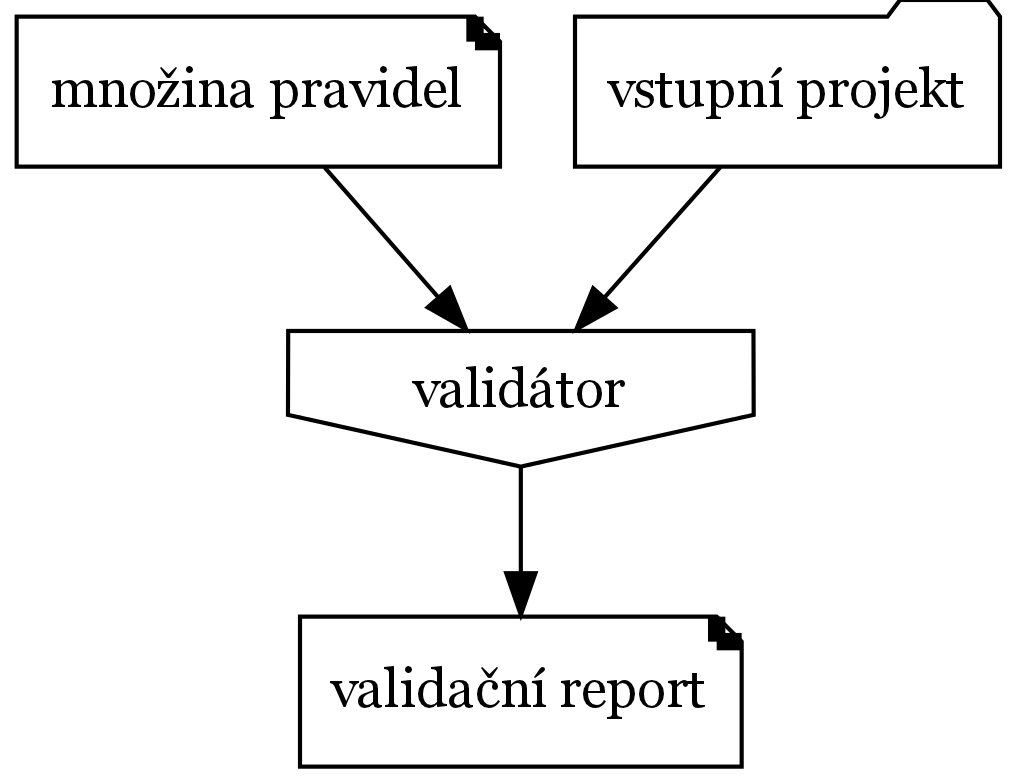
\includegraphics[width=0.5\textwidth]{./graphs/global_structure.png}
  \caption{Struktura systému.\label{requirements-system_structure}}
\end{figure}

Výstupem systému by měl být \emph{validační report}, který vypíše, která pravidla ze vstupního souboru byla porušena. Formát vstupních pravidel a výstupního reportu bude definován dále.

\subsection{Funkční požadavky na výsledný systém}

Na základě obecných požadavků můžeme specifikovat základní funkční požadavky. Požadujeme, aby systém uměl provádět následující funkčnosti:
\begin{itemize}
\item načíst vhodně předzpracovaný projekt a vytvořit vniřní model pro další analýzu,
\item načíst ze vstupního souboru množinu pravidel v definovaném formátu,
\item provést validaci načteného modelu pomocí množiny pravidel,
\item vypsat report obsahující informace o splnění resp. porušení pravidel.
\end{itemize}

\subsection{Nefunkční požadavky na výsledný systém}
Z nefunkčních požadavků můžeme zmínit podporu pro zpracování projektů realizovaných v programovacího jazyce Java. Druhým významným nefunkčním požadavkem je požadavek na rozšiřitelnost. Systém by mělo být možné rozšířit o další modely a možnosti specifikace nových/složitějších pravidel nad modely.

\section{Rešerše existujících řešení}
\label{requirements-existing_tools}

TODO: možná přidat i rešerši exisujících formalizací pro návrh software (Z-notation, UPPAAL, etc.)

TODO: provest resersi o tom, co vsechny tyto nastroje umi, jejich pozitiva a negativa

TODO: v rychlosti zopakovat rešerši na nové nástroje a konkrétní vlastnosti, které jsou důležité pro tuto práci

\subsection{JDepend}

\begin{itemize}
\item \href{http://www.clarkware.com/software/JDepend.html}{http://www.clarkware.com/software/JDepend.html}
\item nástroj pro testování kvality návrhu
\item pracuje nad \verb+*.class+ soubory (získává data z bytekódu)
\end{itemize}

\subsection{QJ-Pro}
\begin{itemize}
\item \href{http://qjpro.sourceforge.net}{http://qjpro.sourceforge.net}
\end{itemize}

\subsection{DP-Miner}
\begin{itemize}
\item \href{http://www.utdallas.edu/~yxz045100/DesignPattern/DP\_Miner/}{http://www.utdallas.edu/~yxz045100/DesignPattern/DP\_Miner/}
\item hledání návrhových vzorů v existujících projektech
\item článek: Jing Dong and Yajing Zhao, Experiments on Design Pattern Discovery \\ (\href{http://www.utdallas.edu/~jdong/papers/PROMISE07.pdf}{http://www.utdallas.edu/~jdong/papers/PROMISE07.pdf})
\end{itemize}

\subsection{Macker}
\begin{itemize}
\item \href{http://innig.net/macker/}{http://innig.net/macker/}
\item build-time architectural rule checking utility for Java developers
\item zpracovává \verb+*.class+ soubory (bytekód)
\end{itemize}

TODO: complete research on following tools:

\subsection{Squale}
\begin{itemize}
\item \href{http://www.squale.org/}{http://www.squale.org/}
\end{itemize}

\subsection{FindBugs}
\begin{itemize}
\item \href{http://findbugs.sourceforge.net/}{http://findbugs.sourceforge.net/}
\end{itemize}

\subsection{CheckStyle}
\begin{itemize}
\item \href{http://checkstyle.sourceforge.net/}{http://checkstyle.sourceforge.net/}
\end{itemize}

\subsection{PMD}
\begin{itemize}
\item \href{http://pmd.sourceforge.net/}{http://pmd.sourceforge.net/}
\end{itemize}

\subsection{Soot}
\begin{itemize}
\item \href{http://www.sable.mcgill.ca/soot/}{http://www.sable.mcgill.ca/soot/}
\item Soot: a Java Optimization Framework
\end{itemize}
